\section{M�todo da vari�vel instrumental - IV}
\label{sec:iv}
%===============================================================================

Uma alternativa para a minimiza��o da polariza��o PPA (propriedades de pequenas
amostras) na estimativa do sistema � a polariza��o assint�tica. A ideia � relaxar
um pouco a defini��o PPA e, por um lado, permitir que haja polariza��o para uma
amostra pequena, mas por outro lado, verificar se tal polariza��o desaparece � 
medida que o tamanho do conjunto de observa��es cresce. \cite{aguirre}

Para utilizac�o deste m�todo, escolhe-se um Instrumento $Z(t)$:

\begin{equation}
Z(t) \in \Re^{p}\; \forall t \;\;\; E(Z(t)\nu)=0
\label{eq:iv_instrumento}
\end{equation}

\begin{equation}
\hat{y}(t, \theta)=\phi ^T (t)\theta
\nonumber
\end{equation}

\begin{equation}
E[Z(t)(y(t)-\hat{y}(t, \theta)]=0
\nonumber
\end{equation}

\begin{equation}
E[Z(t)\phi^T (t)]\theta = E[Z(t)y(t)]
\nonumber
\end{equation}

De onde vem:

\begin{equation}
\hat{\theta}_{N}^{iv}=[\sum_{t=1}^{N}Z(t)\phi^T(t)]^{-1}[\sum_{t=1}^{N}Z(t)y(t)]
\label{eq:iv_estim}
\end{equation}

Ap�s a escolha da estimativa $Z(t)$ que satisfa�a (\ref{eq:iv_estim}) o passo seguinte 
� calcular (\ref{eq:iv_estim_2}).

\begin{equation}
E[\hat{\theta}_{N}^{iv}-\theta_0]=0
\label{eq:iv_estim_2}
\end{equation}


\subsection{M�todo aplicado ao controle de posi��o}
%===============================================================================

Primeiro passo para aplicar o m�todo das {\it{Vari�veis instrumentais}} � escolher
o instrumento que ser� utilizado.

\begin{equation}
\begin{matrix}
w(t)=F(q)u(t)\\
F(q)=q^{-1}\\ 
w(t)=u(t-1)
\end{matrix}
\nonumber
\end{equation}

O que resulta em um instrumento apresentado em (\ref{eq:iv_motor_instr}).

\begin{equation}
Z(t)=\begin{bmatrix}
w(t)\\ 
w(t-1)\\ 
\vdots \\
w(t-p)
\end{bmatrix}
\label{eq:iv_motor_instr}
\end{equation}

No Apendice (\ref{appendix_iv}) encontra-se o script utilizado para as simulac�es deste
m�todo. Foram utilizados os sinais de entrada apresentados nas Figuras (\ref{fig:in_v1_rampa}),
(\ref{fig:in_v2_sin}), (\ref{fig:in_v3_rampa}) e (\ref{fig:in_v4_quad}).

\subsection{Resultados}
%===============================================================================

Os resultados obtidos com a utilizac�o do m�todo das variaveis instrumentais proposrcionou as
estimativas para os parametros $a$ e $b$ que s�o apresentados na Tabela (\ref{tab:iv_results}).

\begin{table}[htbp]
  \begin{center}
	\caption{Valores estimados de $G(q)$ para o m�todo das vari�veis instrumentais}
	\label{tab:iv_results}
	\begin{small}
	  \begin{tabular}{lcll}
		\hline
		Conjunto	& N      & Media a & Media b  \\
		\hline
		1 - Rampa	& 150     &  0.0179 & 0.8771   \\
		1 - Rampa	& 300     &  0.0179 & 0.877    \\
		1 - Rampa	& 600     &  0.018 & 0.8768   \\
		1 - Rampa	& 1500    &  0.018 & 0.8769   \\
		\hline
		2 - Sin 	& 150     & -0.0126 & 1.0739   \\
		2 - Sin 	& 300     & -0.0136 & 1.0796   \\
		2 - Sin 	& 600     & -0.0135 & 1.0789   \\
		2 - Sin 	& 1500    & -0.0137 & 1.0804   \\
		\hline
		3 - Rampa	& 150     & 0.0151  & 0.8962   \\
		3 - Rampa	& 300     & 0.015  & 0.8964   \\
		3 - Rampa	& 600     & 0.0151  & 0.8961   \\
		3 - Rampa	& 1500    & 0.015  & 0.8966   \\
		\hline
		4 - Quadrada & 150    & 0.0113  & 0.8621   \\
		4 - Quadrada & 300    & 0.0114  & 0.8575   \\
		4 - Quadrada & 600    & 0.0114  & 0.8553   \\
		4 - Quadrada & 1500   & 0.0114  & 0.8538   \\
		\hline
	  \end{tabular}
	\end{small}
  \end{center}
\end{table}

A Figura (\ref{fig:iv_d4_quad}) apresenta os valores da estimativa para uma referencia do
tipo onda quadrada (Figura (\ref{fig:in_v4_quad})) utilizando o m�todo das vari�veis 
instrumentais e um conjunto de dados $N=150$.

\begin{figure}[htbp]
	\center
	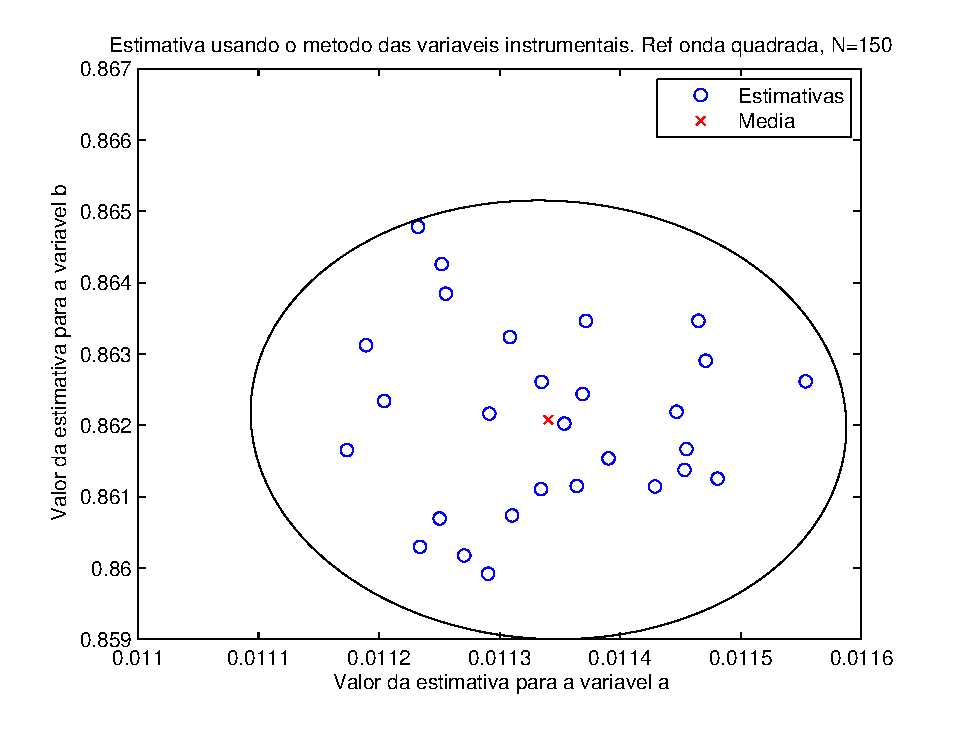
\includegraphics[width=0.98\columnwidth]{figures/iv_d4_quad_n150.eps}
	\caption{Estimativas das vari�veis a e b para o conjunto de dados 4. Utilizando o m�todo
	das vari�veis instrumentais.}
	\label{fig:iv_d4_quad}
\end{figure}


